%&pdflatex
\documentclass{standalone}
\usepackage{tikz}
\usetikzlibrary{arrows}
\usetikzlibrary{shapes}
\usetikzlibrary{positioning}
\usetikzlibrary{snakes}

\begin{document}

\begin{tikzpicture}
\node[inner sep=0pt] (three1) at (-2,3) {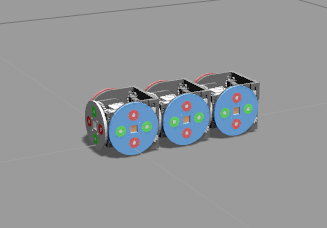
\includegraphics[width=2cm]{../three.png}};
\node[inner sep=0pt] (three2) at (2,3) {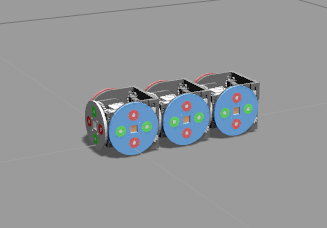
\includegraphics[width=2cm]{../three.png}};
\node[inner sep=0pt] (body) at (0,0) {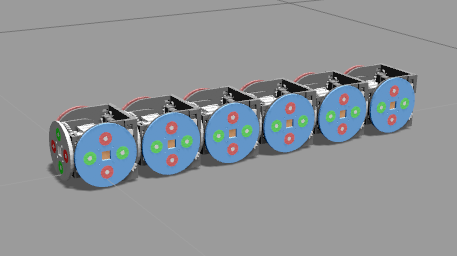
\includegraphics[width=4cm]{../body.png}};
\node[inner sep=0pt] (three3) at (-2,-3) {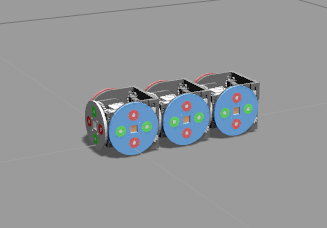
\includegraphics[width=2cm]{../three.png}};
\node[inner sep=0pt] (three4) at (2,-3) {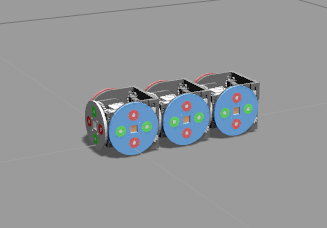
\includegraphics[width=2cm]{../three.png}};
\node[inner sep=0pt] (walkbot) at (6,0) {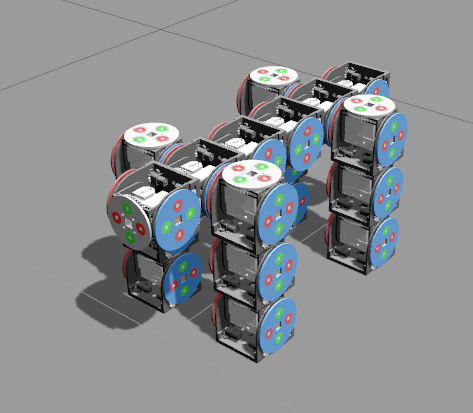
\includegraphics[width=4cm]{../walkbot.png}};

\draw[->,ultra thick] (three1) |-  ([yshift=0.5cm, xshift=-1cm]body.north) -- ([xshift=-0.6cm, yshift=0.4cm]body.center);
\draw[->,ultra thick] (three2) |-  ([yshift=0.5cm, xshift=1cm]body.north) -- ([xshift=0.7cm, yshift=0.7cm]body.center);
\draw[->,ultra thick] (three3) |-  ([yshift=-0.5cm, xshift=-1cm]body.south) -- ([xshift=-0.6cm, yshift=-0.6cm]body.center);
\draw[->,ultra thick] (three4) |-  ([yshift=-0.5cm, xshift=1cm]body.south) -- ([xshift=1cm, yshift=-0.4cm]body.center);
\draw[-implies, double equal sign distance, thick] ([xshift=0.5cm]body.east) -- ([xshift=-0.5cm]walkbot.west);

\end{tikzpicture}

\end{document}



